\documentclass{article}
\usepackage{amsmath,amssymb}
\usepackage{multicol}
\usepackage{graphicx}
\usepackage[margin=1.5in]{geometry}
\setlength{\parskip}{5pt}
\setlength{\parindent}{0pt}
\setlength{\columnseprule}{0.5pt}
\title{Lab 3 work}
\author{20513322}
\date{\today}
\begin{document}
\maketitle
%!!!!!!!!!title title
%!!!!!!!!content content
\tableofcontents
\newpage
\section{Introduction}
%!!!!!!!!!!multicols{2} multicols multicol
\begin{multicols}{2}
he first line of code in any LATEX document is the document class declaration command. It is here that we declare the class of which we like to build our document
\end{multicols}
\underline{add}
\texttt{the}
\section{Different structures}
\subsection{figure}
Below is one example plot of the equation
\begin{equation}
x^3+y^3=3xy
\end{equation}
\begin{figure}[h]
\centering
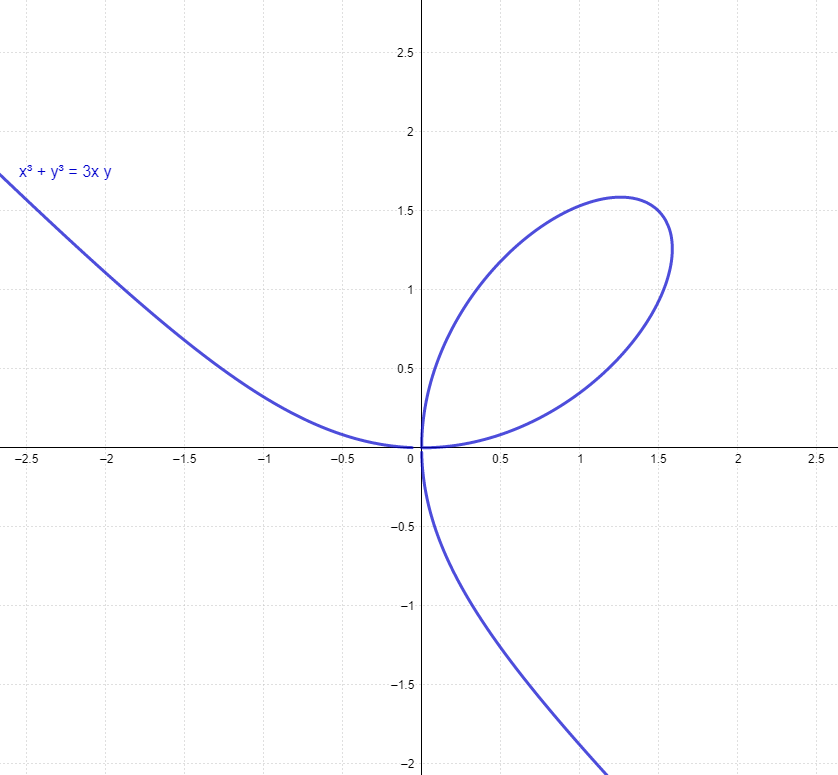
\includegraphics[scale=0.1]{eqnfig}
%!!!!!!!!!!!!!!length is scale
\caption{Folium of Descartes}
\label{1}
\end{figure}
\subsection{List}
\subsubsection{Bulleted list}
\begin{itemize}
\item aritle
\item report
\end{itemize}
%!!!!!!itemize
\subsubsection{Numbered list}
\begin{enumerate}
\item fisrt
\item refence
\end{enumerate}
\subsection{Table}
\begin{itemize}
\item[(a)]  Foundation Calculus
\item[(b)] Introduction to Mathematical Software \& Programming
	\begin{itemize}
	\item[(\#)]\LaTeX
%!!!!!!!!!LaTeX
	\item[(ii)]G
	\item[$iii$]MA
	\end{itemize}
\end{itemize}
\subsection{Math}
\begin{table}[h]
\centering
\begin{tabular}{|l|r|}
\hline
Desciption&Effect\\
noraml&sample\\
bold&\textbf{sam}\\
teletype&\texttt{sam}\\
\hline
\end{tabular}
\caption{Common}
\end{table}
\subsubsection{Example1}
 gg(\ref{1})is here
\begin{equation}
\therefore \frac{2}{x}=2\label{2}
\end{equation}
\subsubsection{Example2}
\ref{2}is here
\end{document}